% Deck Hackathon (21–23 Okt 2026). Kompilasi: latexmk -xelatex main.tex
% Video tertanam (\movie) hanya diputar di Okular, Adobe Reader, atau pdfpc; viewer lain memakai tautan cadangan.
\documentclass[aspectratio=169, 10pt]{beamer}

\usepackage[indonesian]{babel}
\usepackage{fontspec}
\IfFontExistsTF{Calibri}{\setmainfont{Calibri}}{\setmainfont{Carlito}}
\setsansfont{Carlito}
\setmonofont{DejaVu Sans Mono}[Scale=0.8]
\usepackage{tikz}
\usetikzlibrary{positioning,fit,backgrounds,arrows.meta,calc}
\usepackage{pgfplots,pgfplotstable}
\pgfplotsset{compat=1.18}
\usepgfplotslibrary{fillbetween}
\usepackage{booktabs,tabularx,longtable}
\usepackage{qrcode}

% Palet earthy untuk deck (laporan tetap memakai warna jobdesc). Didefinisikan sebelum gaya.tex.
\definecolor{latar}{RGB}{246,240,231}     % linen krem
\definecolor{espresso}{RGB}{78,52,40}     % judul, slide pembuka/penutup
\definecolor{teks}{RGB}{58,46,40}         % teks utama
\definecolor{izma}{RGB}{44,94,104}        % teal-slate
\definecolor{genis}{RGB}{101,122,72}      % hijau zaitun
\definecolor{alif}{RGB}{186,104,64}       % terakota
\definecolor{shania}{RGB}{138,88,112}     % dusty plum
\definecolor{lama}{RGB}{128,116,104}      % abu hangat
\definecolor{merah}{RGB}{168,60,44}       % merah bata
\definecolor{krem}{RGB}{243,232,214}
% Gaya bersama diagram (dipakai laporan progress dan deck). Warna anggota sama dengan jobdesc.tex.
\providecolor{izma}{RGB}{31,94,170}
\providecolor{genis}{RGB}{40,130,70}
\providecolor{alif}{RGB}{190,90,20}
\providecolor{shania}{RGB}{140,60,150}
\providecolor{lama}{RGB}{110,110,110}
\providecolor{merah}{RGB}{185,40,40}
\tikzset{
  kotak/.style={draw, rounded corners=3pt, align=center, font=\footnotesize, inner sep=4pt, line width=0.8pt, minimum height=0.9cm},
  milik/.style={kotak, draw=#1, fill=#1!10},
  abu/.style={kotak, draw=lama, fill=black!4},
  panah/.style={-{Stealth[length=2mm]}, line width=0.7pt, draw=black!70},
  putus/.style={panah, dashed},
  label/.style={font=\scriptsize\itshape, text=black!70, fill=white, inner sep=1pt},
  wadah/.style={draw=#1!60, fill=#1!4, rounded corners=5pt, line width=0.6pt, inner sep=6pt},
}

\newcommand{\diagram}[1]{\input{../diagram/#1.tex}}
% Video tertanam untuk XeLaTeX (xdvipdfmx): poster + anotasi /Movie di atasnya.
% Diputar di Okular/Adobe/pdfpc dengan klik; viewer lain hanya menampilkan poster.
\newcommand{\filmtertanam}[4]{\makebox[#1][l]{\special{pdf:ann width #1 height #2 depth 0pt <</Subtype/Movie /Border [0 0 0]
    /T (video turbin) /Movie <</F (#4) /Aspect [480 848]>> /A <</ShowControls true /Mode /Repeat>> >>}%
  \includegraphics[width=#1,height=#2]{#3}}}
\newcommand{\datafile}[1]{../data/#1}
\graphicspath{{../../proposal/gambar/}{./}}

% ---------- tema sederhana ----------
\usefonttheme{professionalfonts}
\setbeamertemplate{navigation symbols}{}
\setbeamercolor{frametitle}{fg=krem}
\setbeamercolor{structure}{fg=espresso}
\setbeamercolor{normal text}{fg=teks}
\setbeamercolor{background canvas}{bg=white}
\setbeamerfont{frametitle}{size=\Large, series=\bfseries}
% Header: pita espresso selebar halaman + garis terakota; judul krem di dalamnya
\setbeamertemplate{frametitle}{%
  \begin{tikzpicture}[remember picture, overlay]
    \fill[espresso] (current page.north west) rectangle ([yshift=-1.18cm]current page.north east);
    \fill[alif] ([yshift=-1.18cm]current page.north west) rectangle ([yshift=-1.26cm]current page.north east);
  \end{tikzpicture}%
  \vspace{-1pt}\insertframetitle\par\vspace{10pt}}
\setbeamertemplate{itemize item}{\color{alif}\textbullet}
\setbeamertemplate{itemize subitem}{\color{genis}--}
\setbeamertemplate{footline}{\hfill{\scriptsize\color{espresso!55}Tim Chitato \textbullet{} Wind Edge Chip \quad \insertframenumber/\inserttotalframenumber}\hspace{8pt}\vspace{5pt}}
\newcommand{\kriteria}[1]{\hfill{\scriptsize\mdseries\color{krem!75}\textbf{Rubrik:} #1}}
\newcommand{\angka}[3][izma]{\begin{tikzpicture}\node[draw=#1, fill=#1!9, rounded corners=4pt, text width=2.55cm, align=center, inner sep=5pt]
  {{\LARGE\bfseries\color{#1}#2}\\[1pt]{\scriptsize #3}};\end{tikzpicture}}

\ifdefined\wecpitch\setbeamertemplate{footline}{\hfill{\scriptsize\color{espresso!55}Tim Chitato \textbullet{} Wind Edge Chip}\hspace{8pt}\vspace{5pt}}\fi
\ifdefined\wecpitch\includeonlyframes{judul,masalah,solusi,arsitektur,demo,hasil,hil,lebihmaju,bisnis,hilirisasi,penutup}\fi
\begin{document}

% ======================================================================
\begin{frame}[plain,t,label=judul]
\begin{tikzpicture}[remember picture, overlay]
  \fill[espresso] (current page.north west) rectangle ([yshift=-3.7cm]current page.north east);
  \fill[alif] ([yshift=-3.7cm]current page.north west) rectangle ([yshift=-3.82cm]current page.north east);
  \node[anchor=north west, text=krem, font=\fontsize{30}{34}\selectfont\bfseries] at ([xshift=0.9cm, yshift=-0.75cm]current page.north west) {Wind Edge Chip};
  \node[anchor=north west, text=krem!85, text width=9.4cm, font=\large] at ([xshift=0.9cm, yshift=-1.95cm]current page.north west)
    {Prediktor daya turbin angin kecil 1 jam ke depan, berjalan di turbin dengan akselerator INT8 rancangan sendiri};
  \node[anchor=north east, inner sep=0, draw=white, line width=2pt] at ([xshift=-0.7cm, yshift=-0.55cm]current page.north east)
    {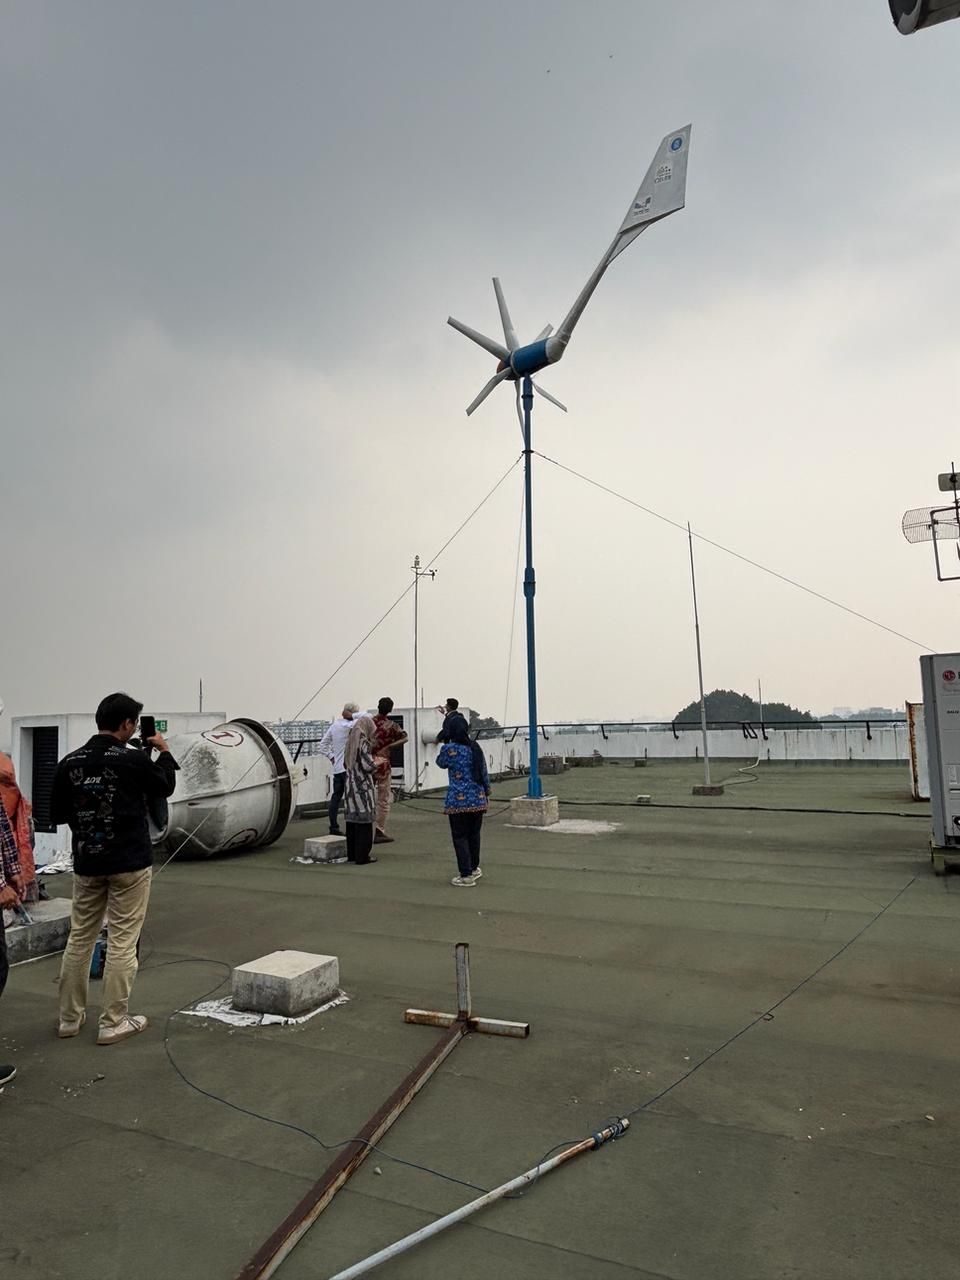
\includegraphics[height=5.6cm]{foto-turbin-atap.jpeg}};
  \node[anchor=north west, text width=9.6cm, align=left, text=teks] at ([xshift=0.9cm, yshift=-4.35cm]current page.north west) {%
    {\small\color{alif}\textbf{DeepTech for Smart-X Hackathon 2026}}\\[1pt]
    {\small Renewable Energy \textbullet{} Wind Power Output Forecasting}\\[12pt]
    {\small\textbf{\color{espresso}Tim Chitato}}\\[2pt]
    {\small Izma Alhazmi Herdian (ketua) \textbullet{} Genis Gusvian Hartanto\\Alif Muhammad Rizky \textbullet{} Shania Argiliana}\\[6pt]
    {\small\textbf{\color{espresso}Pembimbing:} Ir.\ Estiyanti Ekawati, M.T., Ph.D.}};
\end{tikzpicture}
\end{frame}

% ======================================================================
\begin{frame}[label=masalah]{Masalah: daya turbin kecil tak terduga\kriteria{problem-solution fit (20\%)}}
\begin{columns}[T]
\begin{column}{0.55\linewidth}
\begin{itemize}
  \item Turbin di atap Gedung CRIMSE ITB: daya \textbf{0 W} di malam hari (88\% menit OFF pukul 00--06) sampai \textbf{$>$100 W} di sore yang berangin.
  \item Pengelola \textbf{tidak punya dasar} memutuskan kapan listrik diisikan ke baterai, kapan beban dinyalakan, dan kapan beralih ke PLN.
  \item Sistem saat ini (Raspi + internet + Google Sheets) \textbf{kehilangan data saat internet mati}.
  \item \textbf{Masukan mitra PLN} (coaching clinic 16 Okt): forecasting daya sudah ada di PLN; yang belum ada adalah prediksi \textbf{setelah inverter / ke baterai}.
\end{itemize}
\end{column}
\begin{column}{0.43\linewidth}
\begin{tikzpicture}
\begin{axis}[width=\linewidth, height=4.6cm, ybar, bar width=3pt, xlabel={jam (WIB)}, ylabel={\% menit OFF}, ymin=0, ymax=100,
             xtick={0,6,12,18}, tick label style={font=\tiny}, label style={font=\scriptsize}, title={\scriptsize Turbin diam sebagian besar malam}]
  \addplot[fill=izma!60, draw=izma] table[col sep=comma, x=jam, y=off_persen] {\datafile{off_per_jam.csv}};
\end{axis}
\end{tikzpicture}
\end{column}
\end{columns}
\end{frame}

% ======================================================================
\begin{frame}[label=solusi]{Solusi: prediksi di turbin, dalam tiga lapis\kriteria{inovasi \& kebaruan (15\%)}}
\centering
\begin{tikzpicture}[node distance=0.4cm and 0.5cm]
  \node[milik=genis, text width=4.2cm, minimum height=2.6cm] (l1) {\textbf{L1 Digitalisasi}\\[3pt]\footnotesize ESP32 baca sensor, buffer lokal, MQTT\\Node-RED + database\\dashboard: daya aktual vs prediksi 1 jam};
  \node[milik=izma, text width=4.2cm, minimum height=2.6cm, right=of l1] (l2) {\textbf{L2 Edge AI}\\[3pt]\footnotesize MLP 16-32-16-1 \textbf{INT8}\\dilatih dengan aritmetika chip\\tetap jalan tanpa internet};
  \node[milik=alif, text width=4.2cm, minimum height=2.6cm, right=of l2] (l3) {\textbf{L3 Semikonduktor}\\[3pt]\footnotesize akselerator MAC4 paralel di FPGA\\RTL sendiri, 309 siklus/prediksi\\jalur ke ASIC (OpenLane/SKY130)};
  \draw[panah] (l1) -- (l2); \draw[panah] (l2) -- (l3);
\end{tikzpicture}

\vspace{8pt}
\begin{tikzpicture}
  \node[draw=shania, fill=shania!8, rounded corners=4pt, text width=13cm, align=center, font=\small, inner sep=6pt]
  {\textbf{Keluaran:} rata-rata daya 60 menit ke depan (= energi jam depan) + interval P10--P90 $\to$ energi masuk baterai dan SoC 1 jam lagi $\to$ keputusan isi baterai / beban / PLN};
\end{tikzpicture}
\end{frame}

% ======================================================================
\begin{frame}[label=arsitektur]{Arsitektur sistem\kriteria{fungsional prototipe (25\%)}}
\centering\resizebox{\linewidth}{!}{\diagram{arsitektur}}
\end{frame}

% ======================================================================
\begin{frame}[label=demo]{Demo live (3 menit)\kriteria{fungsional prototipe (25\%)}}
\begin{columns}[T]
\begin{column}{0.62\linewidth}
\small
\begin{enumerate}
  \item \textbf{Dashboard} \texttt{citaitb.com:1880/dashboard/hackathon}: data turbin di atap CRIMSE detik ini, prediksi 1 jam + rentang 80\%.
  \item \textbf{Chip di meja}: ESP32-S3 $\to$ Tang Nano 4K menghitung prediksi yang sama; baris ``Chip: Tang Nano 4K aktif'', hasil identik dengan CPU, 309 siklus.
  \item \textbf{Status \& baterai}: daya aktual vs daya wajar; SoC 1 jam ke depan $\to$ kapan perlu PLN.
  \item \textbf{Ketahanan}: mode cadangan saat PZEM diam, mode celah saat Raspi reboot.
  \item \textbf{Digital twin}: geser angin, model INT8 yang sama di browser.
  \item \textbf{Daya komputasi}: Raspberry Pi vs FPGA + ESP32-S3 (INA219, live).
\end{enumerate}
\end{column}
\begin{column}{0.36\linewidth}
\centering
\qrcode[height=3.2cm]{http://citaitb.com:1880/dashboard/hackathon}\\[4pt]
{\scriptsize Pindai untuk ikut membuka di ponsel}\\[8pt]
\begin{tikzpicture}
  \node[draw=alif, fill=alif!8, rounded corners=4pt, text width=4.6cm, align=left, font=\scriptsize, inner sep=5pt]
  {\textbf{Cadangan bila internet putus:} video turbin, tangkapan layar dashboard (slide sebelumnya), uji HIL di papan lewat USB.};
\end{tikzpicture}
\end{column}
\end{columns}
\end{frame}

% ======================================================================
\begin{frame}{Sistem nyata di lapangan\kriteria{problem-solution fit}}
\begin{columns}[T]
\begin{column}{0.27\linewidth}
\centering
\filmtertanam{3.45cm}{6.1cm}{poster-video.jpg}{video-turbin.mp4}\\[3pt]
{\tiny Klik untuk memutar (Okular/Adobe/pdfpc).\\Cadangan: \href{run:video-turbin.mp4}{\color{izma}buka video-turbin.mp4}}
\end{column}
\begin{column}{0.71\linewidth}
\centering\resizebox{\linewidth}{!}{\diagram{topologi}}\\[8pt]
\small Sistem monitoring TA (TKT 5--6) sudah berjalan di atap Gedung CRIMSE: PZEM-017, stasiun cuaca, Raspi 4,
MQTT tiap 3 detik, Node-RED, Google Sheets, dan dashboard HMI yang bisa dibuka publik (slide berikut).
\end{column}
\end{columns}
\end{frame}

% ======================================================================
\begin{frame}[label=dashboard]{Dashboard: data live + tiga fitur ML (Node-RED)\kriteria{fungsional prototipe (25\%)}}
\begin{columns}[T]
\begin{column}{0.66\linewidth}
\centering
\href{http://citaitb.com:1880/dashboard/hackathon}{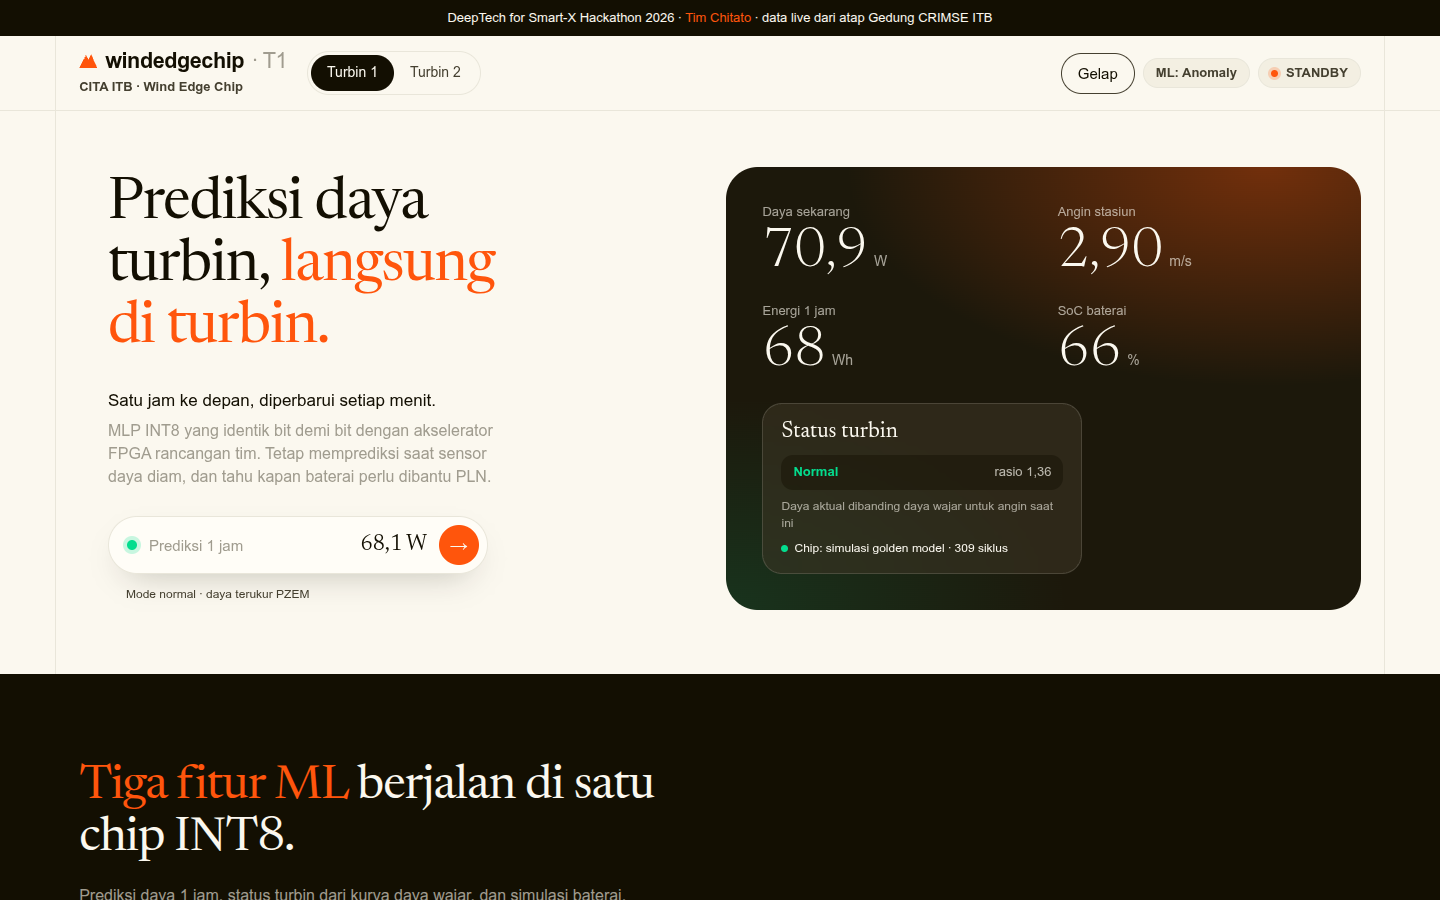
\includegraphics[width=\linewidth]{../gambar/hmi-hackathon-2026-10-21.png}}\\[2pt]
{\tiny Tangkapan live \texttt{/dashboard/hackathon}, 21 Okt 2026 08.32 WIB: prediksi 1 jam 68,1 W (rentang 41--72 W), status Normal (klik untuk membuka).}\\[4pt]
\scriptsize Mesin ML di Node-RED (MLP INT8 \textbf{identik FPGA}) tiap menit: prediksi 1 jam + P10--P90, status, SoC baterai;
CCTV berdampingan dengan \textbf{digital twin 3D}; riwayat di \textbf{InfluxDB}.
\end{column}
\begin{column}{0.32\linewidth}
\centering
\textbf{\small Buka tanpa login}\\[4pt]
\begin{tikzpicture}
  \node[milik=genis, text width=4.1cm, align=left, font=\scriptsize] {%
    \href{http://citaitb.com:1880/dashboard/hackathon}{\color{genis!60!black}\texttt{citaitb.com:1880/}\\\texttt{dashboard/hackathon}}\\[2pt]
    IP: \href{http://103.102.153.154:1880/dashboard/hackathon}{\color{genis!60!black}\texttt{103.102.153.154:1880}}};
\end{tikzpicture}\\[6pt]
\qrcode[height=3.1cm]{http://citaitb.com:1880/dashboard/hackathon}\\[3pt]
{\tiny Pindai untuk membuka di ponsel.\\Pemuatan pertama $\pm$10--15 detik.}
\end{column}
\end{columns}
\end{frame}

% ======================================================================
\begin{frame}{Dashboard: tiga fitur ML, live\kriteria{fungsional prototipe}}
\begin{columns}[T]
\begin{column}{0.6\linewidth}
\centering\href{http://citaitb.com:1880/dashboard/hackathon}{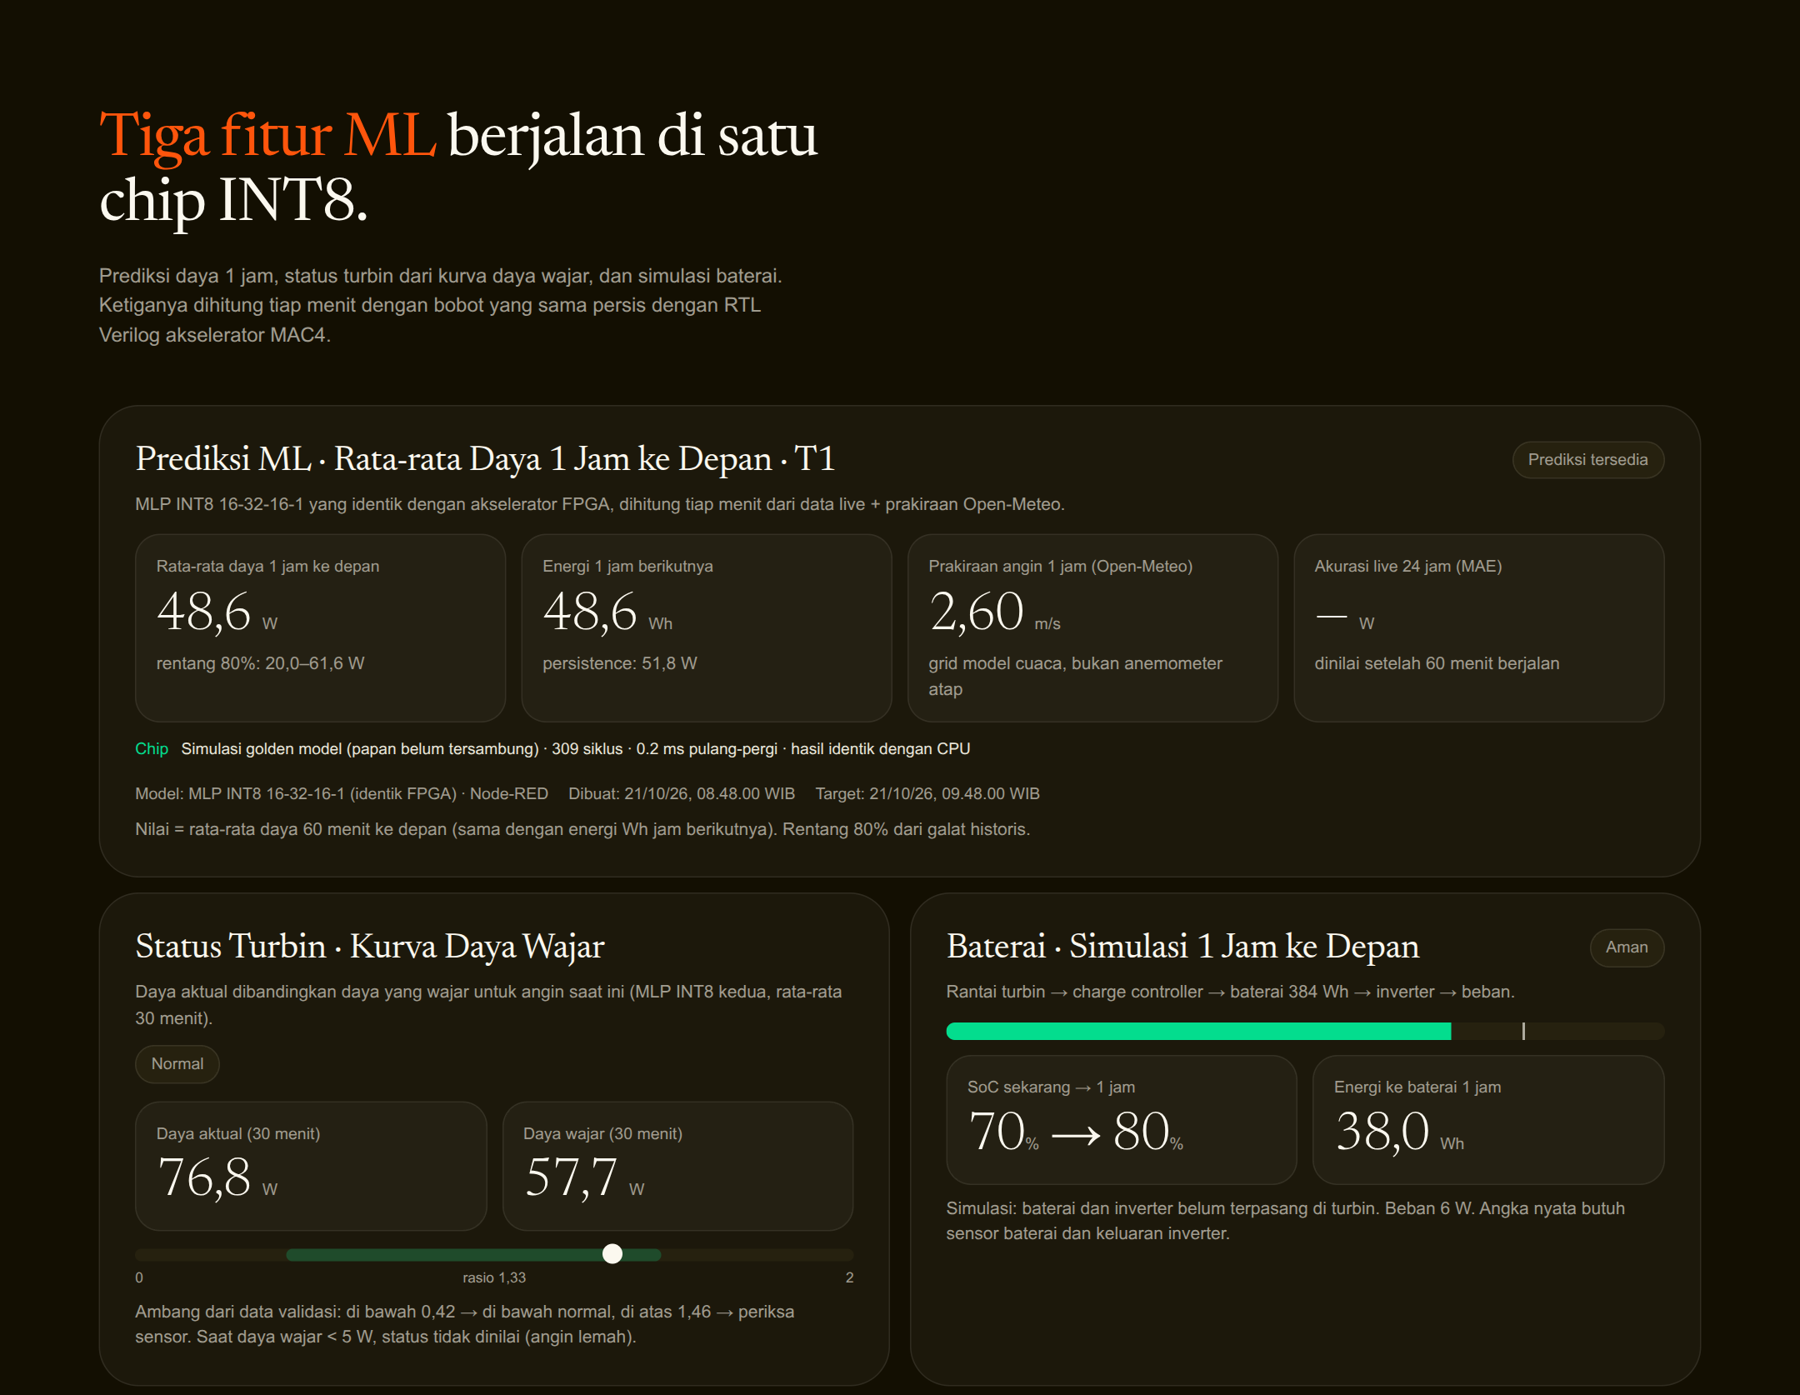
\includegraphics[width=\linewidth]{../gambar/dash-ml-band.png}}\\[2pt]
{\tiny Tangkapan live 21 Okt 2026 08.48 WIB.}
\end{column}
\begin{column}{0.38\linewidth}
\footnotesize
\begin{itemize}
  \item \textbf{Prediksi 1 jam} + rentang 80\% (P10--P90), energi Wh, prakiraan angin Open-Meteo, akurasi live 24 jam.
  \item \textbf{Chip}: 16 fitur INT8 yang sama dikirim ke akselerator (paket + CRC-8); 309 siklus, hasil \textbf{identik} dengan CPU.
  \item \textbf{Status turbin}: daya aktual vs daya wajar (MLP INT8 kedua), rasio 30 menit dengan ambang validasi.
  \item \textbf{Baterai}: SoC sekarang $\to$ 1 jam lagi dan energi masuk baterai (simulasi aki 12 V 50 Ah).
\end{itemize}
\end{column}
\end{columns}
\end{frame}

% ======================================================================
\begin{frame}{Dashboard: data sensor, CCTV, dan digital twin\kriteria{fungsional prototipe}}
\begin{columns}[T]
\begin{column}{0.56\linewidth}
\centering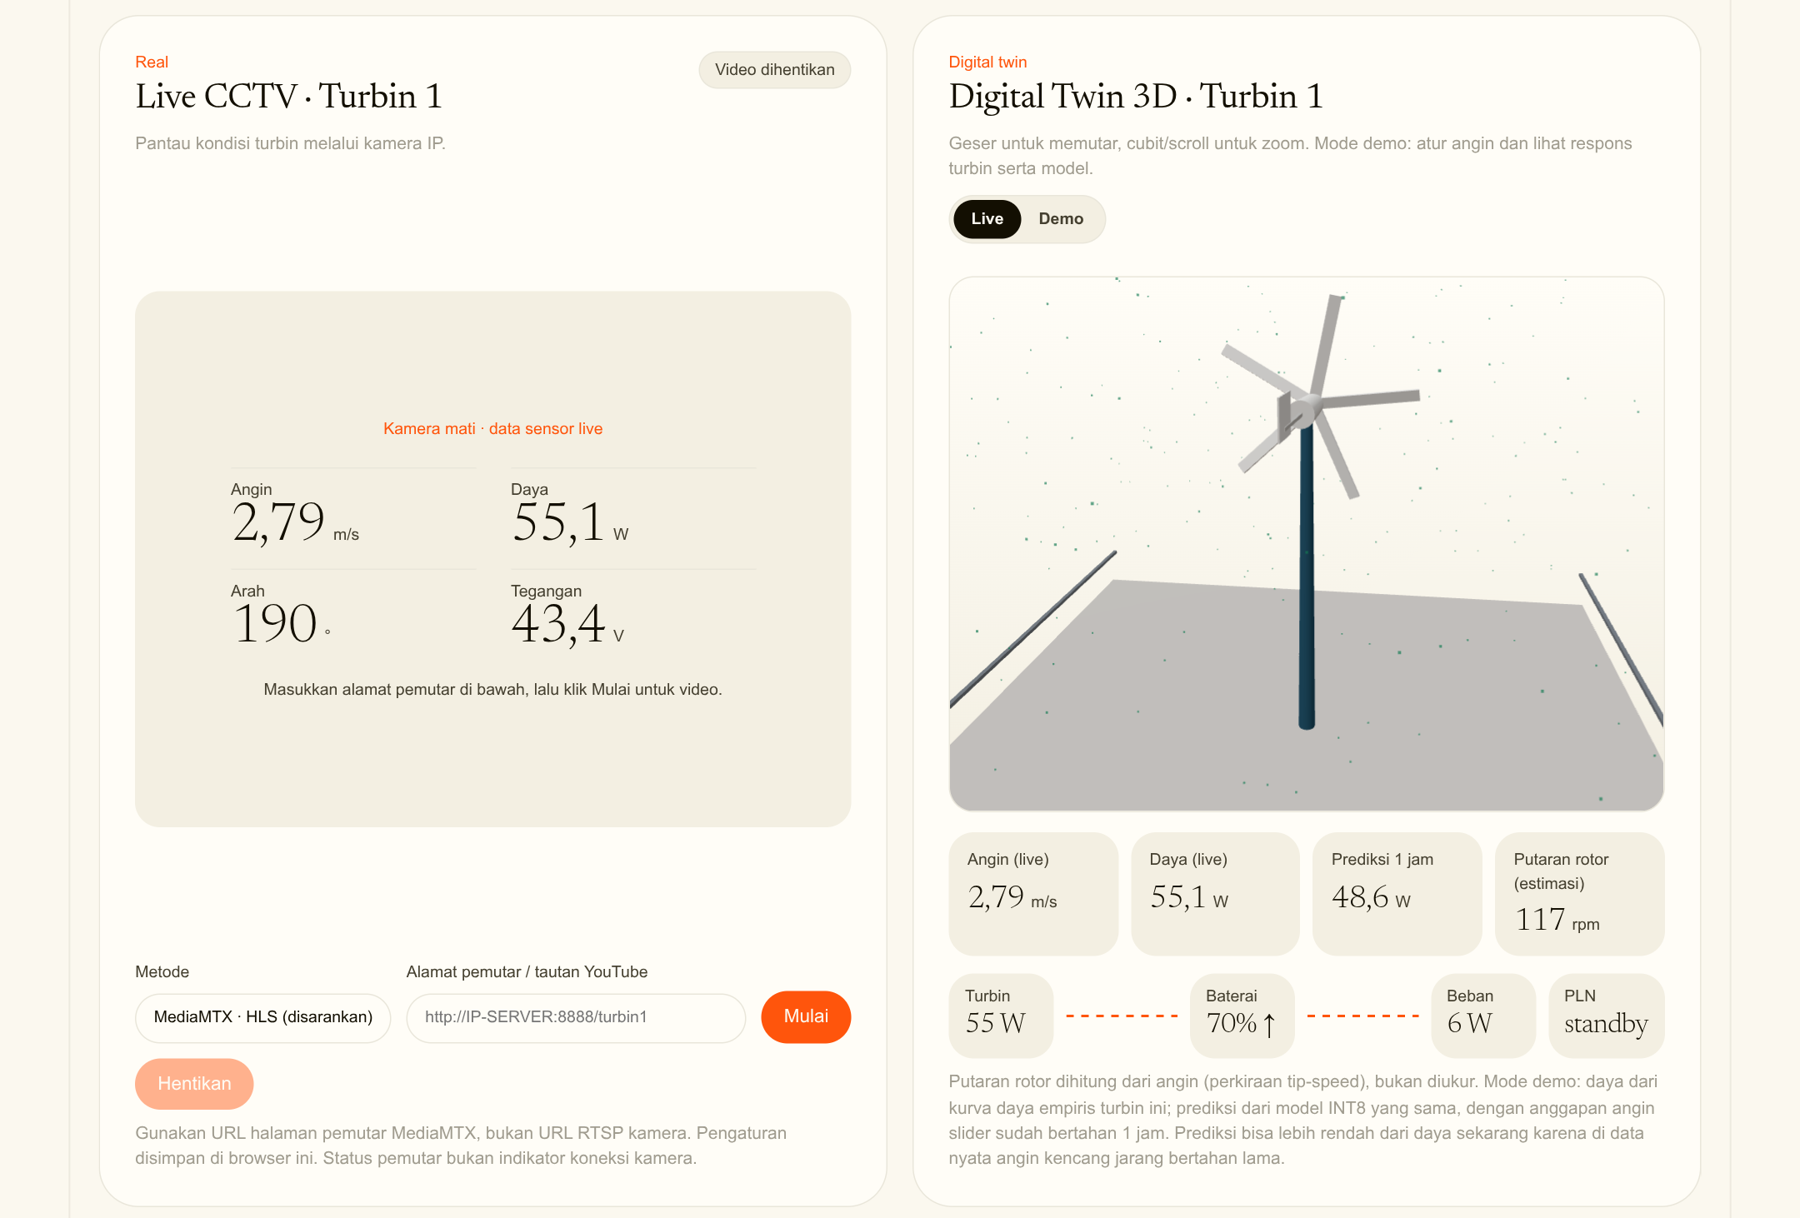
\includegraphics[width=\linewidth]{../gambar/dash-compare.png}\\[2pt]
{\tiny Kiri: kamera/data sensor live. Kanan: digital twin 3D (mode Live/Demo) + aliran energi.}
\end{column}
\begin{column}{0.42\linewidth}
\centering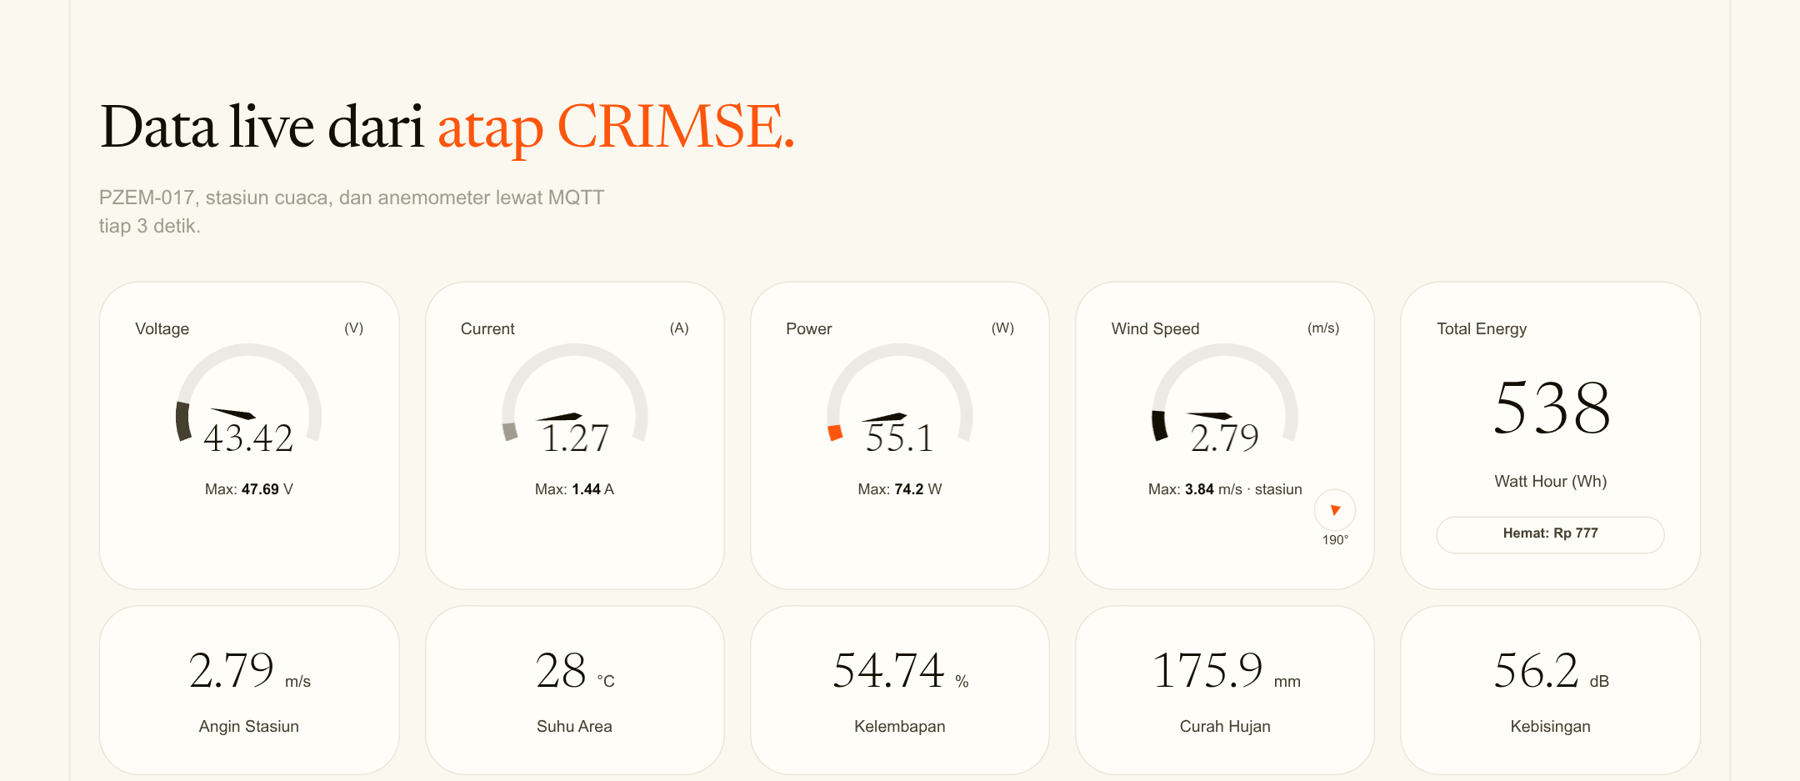
\includegraphics[width=\linewidth]{../gambar/dash-live.png}\\[2pt]
{\tiny PZEM-017 + stasiun cuaca tiap 3 detik (angin = stasiun; anemometer Arduino macet di 1,25 m/s).}\\[6pt]
\footnotesize\raggedright
\begin{itemize}
  \item Mode \textbf{Demo}: geser angin, daya dari kurva empiris, prediksi dari model INT8 yang sama di browser.
  \item Rotor, arah yaw, dan partikel angin mengikuti data live.
\end{itemize}
\end{column}
\end{columns}
\end{frame}

% ======================================================================
\begin{frame}{Dashboard di ponsel dan database riwayat\kriteria{fungsional prototipe}}
\begin{columns}[T]
\begin{column}{0.22\linewidth}
\centering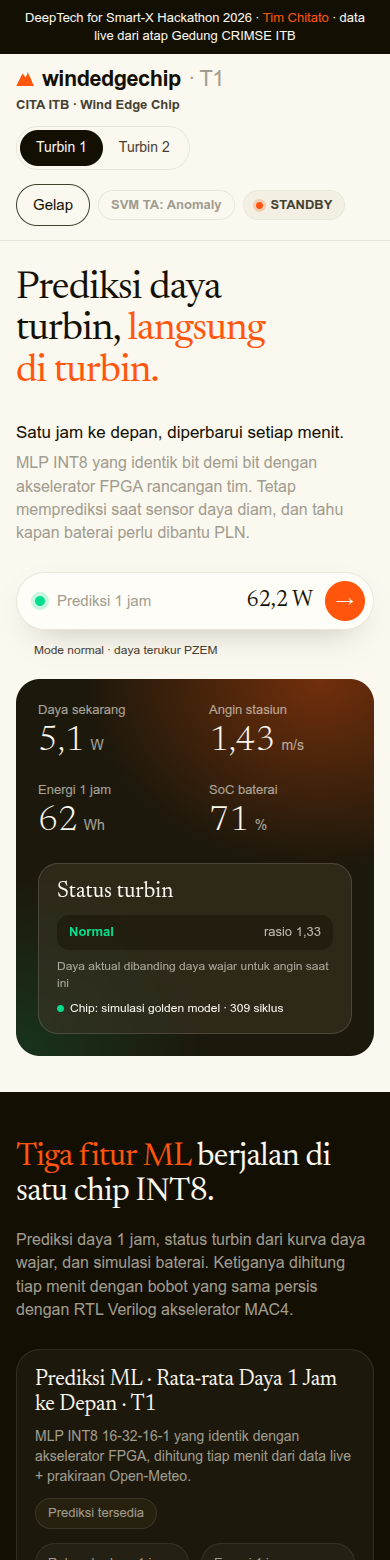
\includegraphics[height=6.3cm]{../gambar/dash-hp.png}\\[2pt]
{\tiny Tampilan HP (390 px).}
\end{column}
\begin{column}{0.76\linewidth}
\centering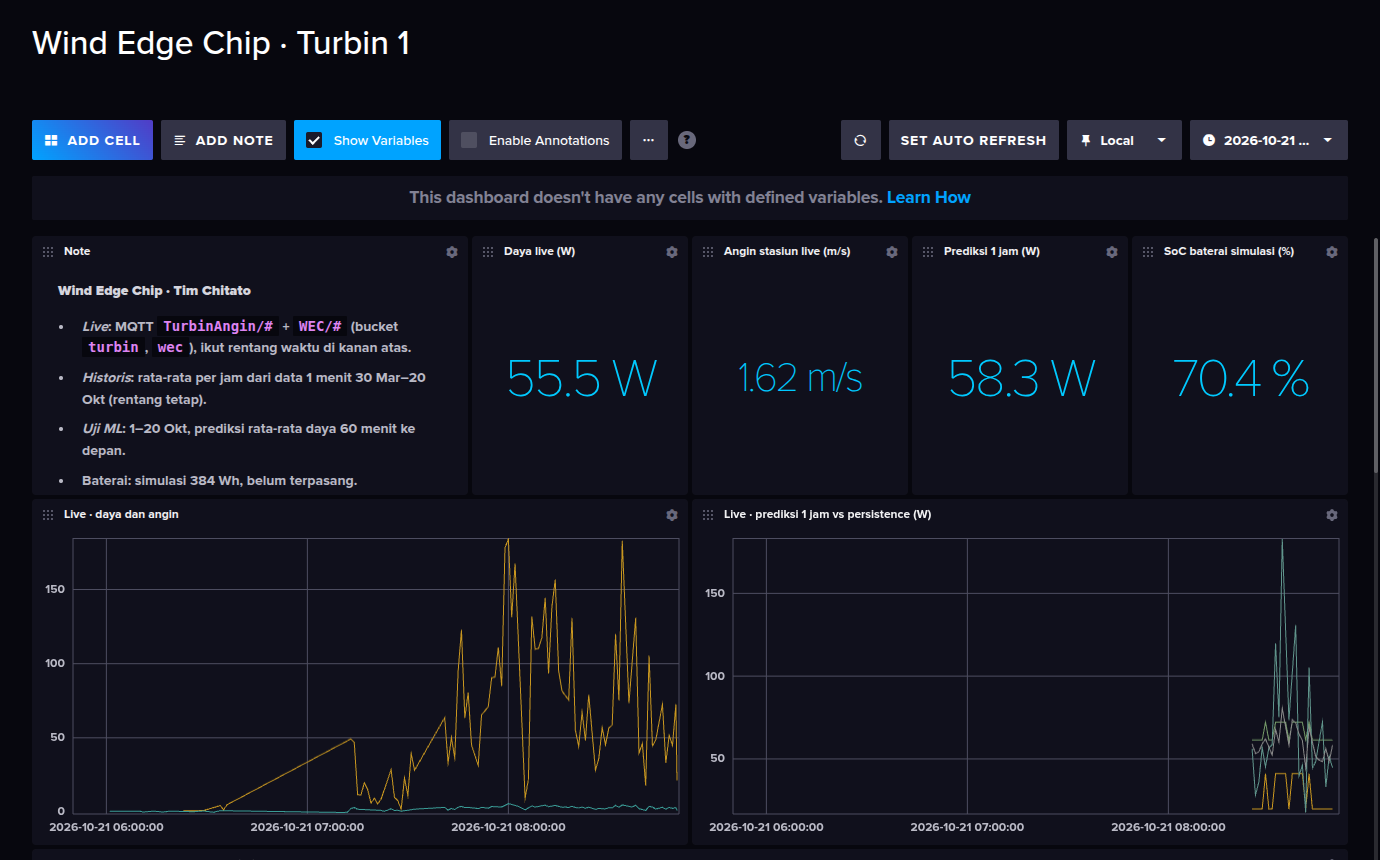
\includegraphics[height=5.6cm]{../gambar/dash-influx.png}\\[2pt]
{\tiny InfluxDB: daya + angin live, prediksi vs persistence, historis 181 rb menit, uji 1--20 Okt, SoC, hasil chip.}\\[3pt]
\scriptsize Google Sheets TA tetap jalan; InfluxDB menambah query per waktu tanpa batas 10 juta sel.
\end{column}
\end{columns}
\end{frame}

% ======================================================================
\begin{frame}{Data nyata: 2,2 juta baris, dibersihkan dengan jujur\kriteria{problem-solution fit}}
\begin{columns}[T]
\begin{column}{0.5\linewidth}
\begin{itemize}\small
  \item 13 Jan--20 Okt 2026; dipakai \textbf{30 Mar--20 Okt} (ada angin stasiun) $\to$ \textbf{181.228 menit} bersih.
  \item Temuan dan perbaikan:
  \begin{itemize}\footnotesize
    \item Excel mengubah angka jadi tanggal (\texttt{28.4} $\to$ 28 April): Suhu 334 rb, Daya 119 rb sel. Daya \textbf{dipulihkan} dari V$\times$I (galat 1,1\%).
    \item Anemometer Arduino macet di 1,25 m/s (42\%) $\to$ pakai angin stasiun.
    \item \texttt{OFF} = turbin tidak menghasilkan (angin 0,7 vs 2,3 m/s) $\to$ 0 W.
    \item Celah data akibat internet mati $\to$ tidak diinterpolasi.
  \end{itemize}
\end{itemize}
\end{column}
\begin{column}{0.48\linewidth}
\begin{tikzpicture}
\begin{axis}[width=\linewidth, height=3.6cm, ybar, bar width=6pt, symbolic x coords={Mar,Apr,Mei,Jun,Jul,Agu,Sep,Okt}, xtick=data,
             ylabel={jam data}, axis y line*=left, ymin=0, tick label style={font=\tiny}, label style={font=\scriptsize}, enlarge x limits=0.08]
  \addplot[fill=genis!60, draw=genis] table[col sep=comma, x=bulan, y=jam_data] {\datafile{data_per_bulan.csv}};
\end{axis}
\begin{axis}[width=\linewidth, height=3.6cm, symbolic x coords={Mar,Apr,Mei,Jun,Jul,Agu,Sep,Okt}, xtick=\empty, ylabel={reboot}, axis y line*=right,
             axis x line=none, ymin=0, tick label style={font=\tiny}, label style={font=\scriptsize, text=merah}, enlarge x limits=0.08]
  \addplot[merah, thick, mark=*, mark size=1.2pt] table[col sep=comma, x=bulan, y=reboot] {\datafile{data_per_bulan.csv}};
\end{axis}
\end{tikzpicture}\\
\begin{tikzpicture}
\begin{axis}[width=\linewidth, height=3.3cm, xlabel={angin (m/s)}, ylabel={daya (W)}, ymin=0, tick label style={font=\tiny}, label style={font=\scriptsize}]
  \addplot[izma, mark=*, mark size=1pt] table[col sep=comma, x=angin, y=mean] {\datafile{kurva_daya.csv}};
\end{axis}
\end{tikzpicture}
\end{column}
\end{columns}
\end{frame}

% ======================================================================
\begin{frame}{Edge AI: pipeline dan tiga fitur ML\kriteria{inovasi \& kebaruan}}
\centering\resizebox{0.95\linewidth}{!}{\diagram{pipeline}}

\vspace{6pt}
\begin{tabularx}{\linewidth}{@{}l X@{}}
\toprule
\textbf{1. Status turbin} & MLP INT8 \textbf{kurva daya wajar} (topologi sama, lulus RTL) $\to$ rasio aktual/wajar 30 menit; SVM TA direproduksi (97,6\%) \\
\textbf{2. Prediksi daya 1 jam} & 16 fitur (lag daya, angin, $v^3$, arah, jam, $\rho$, prakiraan Open-Meteo) $\to$ MLP INT8 di FPGA \\
\textbf{3. Baterai/inverter} & rantai daya DC $\to$ charge controller $\to$ baterai $\to$ inverter (masukan PLN) \\
\bottomrule
\end{tabularx}
\end{frame}

% ======================================================================
\begin{frame}[label=hasil]{Hasil prediksi 1 jam (uji 1--20 Okt)\kriteria{problem-solution fit (20\%)}}
\begin{columns}[T]
\begin{column}{0.36\linewidth}
\centering
\angka{10,25 W}{RMSE MLP INT8 (FPGA)}\\[4pt]
\angka[genis]{+0,40}{skill vs persistence}\\[4pt]
\angka[alif]{0 beda}{golden model vs RTL\\597 vektor uji}\\[4pt]
\IfFileExists{../data/benchmark_jumlah.tex}{{\scriptsize36 metode dibandingkan; MLP INT8 peringkat 6. Terbaik: Transformer (riwayat 60 menit) (10,07 W).}}{}
\end{column}
\begin{column}{0.62\linewidth}
\IfFileExists{../data/benchmark_top.csv}{%
\pgfplotstableread[col sep=semicolon]{\datafile{benchmark_top.csv}}\toptable
\begin{tikzpicture}
\begin{axis}[width=0.36\linewidth, scale only axis, height=5.6cm, xbar, bar width=5pt, xlabel={RMSE (W), makin kecil makin baik}, xmin=0, xmax=18,
             ytick=data, yticklabels from table={\toptable}{label}, y dir=reverse,
             yticklabel style={font=\scriptsize}, xticklabel style={font=\scriptsize}, label style={font=\scriptsize}, enlarge y limits=0.04,
             xtick={0,5,10,15}]
  \addplot[fill=izma!55, draw=izma] table[x=RMSE_W, y expr=\coordindex] {\toptable};
\end{axis}
\end{tikzpicture}}{}
\end{column}
\end{columns}
\end{frame}

% ======================================================================
\begin{frame}{Contoh prediksi dua hari\kriteria{problem-solution fit}}
\centering
\begin{tikzpicture}
\begin{axis}[width=\linewidth, height=6.2cm, xlabel={jam sejak 00.00 WIB, \input{../data/contoh_prediksi_tanggal.txt}}, ylabel={daya rata-rata 1 jam ke depan (W)},
             ymin=0, xmin=0, xmax=48, xtick={0,6,...,48}, tick label style={font=\scriptsize}, label style={font=\scriptsize},
             legend style={font=\scriptsize, at={(0.99,0.98)}, anchor=north east}]
  \addplot[name path=lo, draw=none, forget plot] table[col sep=comma, x=jam, y=p10] {\datafile{contoh_prediksi.csv}};
  \addplot[name path=hi, draw=none, forget plot] table[col sep=comma, x=jam, y=p90] {\datafile{contoh_prediksi.csv}};
  \addplot[izma!15, forget plot] fill between[of=lo and hi];
  \addplot[black, thick] table[col sep=comma, x=jam, y=aktual] {\datafile{contoh_prediksi.csv}};
  \addplot[lama, dashed] table[col sep=comma, x=jam, y=persistence] {\datafile{contoh_prediksi.csv}};
  \addplot[izma, thick] table[col sep=comma, x=jam, y=int8] {\datafile{contoh_prediksi.csv}};
  \legend{aktual, persistence, MLP INT8 (FPGA)}
\end{axis}
\end{tikzpicture}\\
{\scriptsize Area teal muda = interval P10--P90 (model kuantil): ketidakpastian ikut dilaporkan.}
\end{frame}

% ======================================================================
\begin{frame}[label=chip]{Chip L3: akselerator MAC4 rancangan sendiri\kriteria{inovasi \& kebaruan (15\%)}}
\centering\resizebox{0.9\linewidth}{!}{\diagram{mac4}}\\[10pt]
\begin{tikzpicture}
  \node[milik=alif, text width=3.6cm] (a) {\textbf{1.040 MAC INT8}\\260 langkah MAC4};
  \node[milik=alif, text width=3.6cm, right=0.5cm of a] (b) {\textbf{309 siklus}\\$\approx$11,4\,$\mu$s pada 27 MHz};
  \node[milik=alif, text width=3.6cm, right=0.5cm of b] (c) {\textbf{Tang Nano 4K}\\LUT 24\% \textbullet{} Fmax 85,7 MHz};
\end{tikzpicture}
\end{frame}

\begin{frame}{Model dilatih dengan aritmetika chip\kriteria{inovasi \& kebaruan}}
\centering\resizebox{0.86\linewidth}{!}{\diagram{fpga_alur}}\\[8pt]
\resizebox{\linewidth}{!}{\diagram{verifikasi}}\\[6pt]
\small Bobot hasil latih langsung menjadi \texttt{weights32.hex}; setiap neuron sama persis dengan RTL Verilog,
lalu ditanam di bitstream dan di-flash ke Tang Nano 4K.
\end{frame}

% ======================================================================
\begin{frame}{Hasil FPGA: prediksi RTL vs data aktual\kriteria{fungsional prototipe}}
% Dibuat oleh ml/results/export_rtl_predictions.py; jangan diedit manual.
\newcommand{\RtlN}{597}
\newcommand{\RtlMismatch}{0}
\newcommand{\RtlCycles}{309}
\newcommand{\RtlMae}{9.45}
\newcommand{\RtlRmse}{19.25}

\begin{columns}[T]
\begin{column}{0.65\linewidth}
\centering
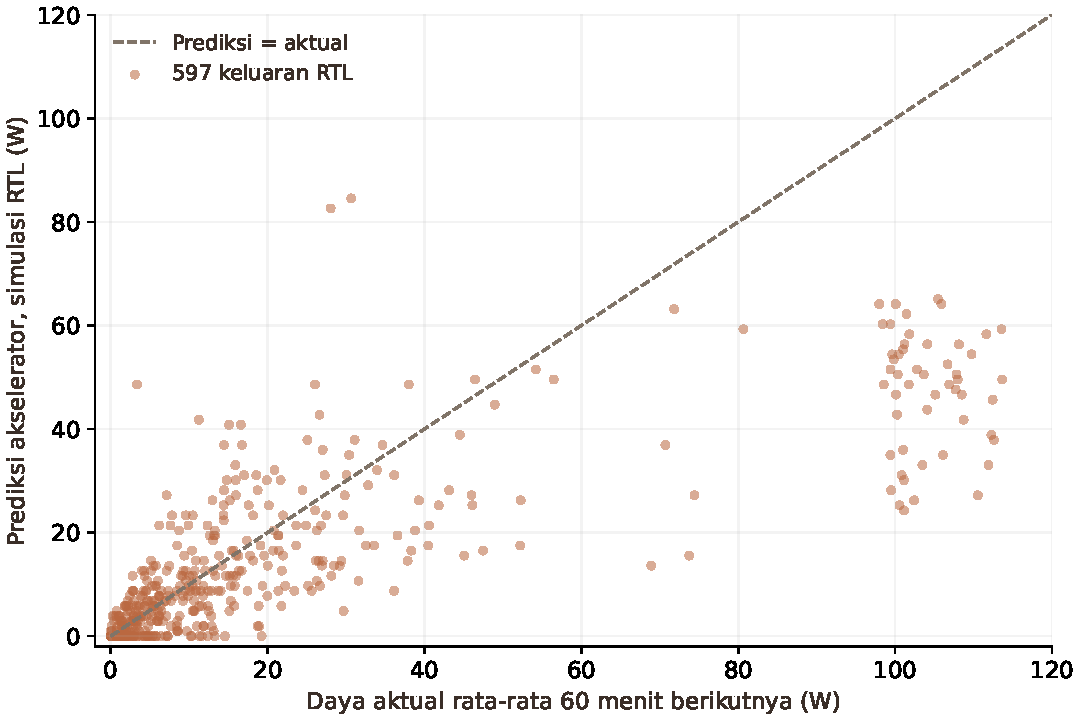
\includegraphics[width=0.94\linewidth]{../gambar/prediksi-rtl.pdf}\\[-2pt]
{\scriptsize Target = rata-rata daya 60 menit berikutnya.\\
MAE subset \RtlMae\ W; RMSE subset \RtlRmse\ W.}
\end{column}
\begin{column}{0.33\linewidth}
\centering
\angka[alif]{\RtlMismatch\ beda}{RTL vs golden model\\\RtlN\ sampel nyata}\\[3pt]
\small\textbf{\RtlCycles\ siklus per prediksi}\\
{\scriptsize $\approx$11,4\,$\mu$s pada 27 MHz}\\[7pt]
\scriptsize
\begin{tabular}{@{}l r@{}}
\toprule
\multicolumn{2}{@{}l}{\textbf{Tang Nano 4K (laporan Alif)}}\\
\midrule
Logika LUT + ALU & 24\% \\
DSP & 2 / 8 \\
BSRAM & 1 / 10 \\
Daya (estimasi) & $\approx$26,9 mW \\
\bottomrule
\end{tabular}
\end{column}
\end{columns}
\vspace{2pt}
{\tiny Simulasi Icarus Verilog; hasil di papan sama persis (slide berikut). Subset: 550 indeks acak + 50 target tertinggi (597 unik).\\
Metrik subset berbeda dari seluruh 16.255 menit uji. Daya: estimasi laporan Alif.}
\end{frame}

% ======================================================================
\begin{frame}[label=hil]{Chip jalan di papan: uji HIL 21 Okt\kriteria{fungsional prototipe (25\%)}}
\begin{columns}[T]
\begin{column}{0.42\linewidth}
\small\textbf{ESP32-S3 $\leftrightarrow$ Tang Nano 4K}\\[4pt]
\footnotesize
\begin{tabularx}{\linewidth}{@{}X r@{}}
\toprule
Inferensi di papan identik dengan golden model + CPU ESP32 & \textbf{\color{alif}5.373/5.373} \\
Ronde uji (597 vektor nyata tiap ronde) & 9 \\
Siklus hitung & \textbf{309} (11,4\,$\mu$s) \\
Pulang-pergi UART 921600 (19 B + 7 B) & 482\,$\mu$s \\
Paket hilang / CRC salah / coba ulang & 0 / 0 / 0 \\
\bottomrule
\end{tabularx}\\[6pt]
\scriptsize Bitstream RTL 21 Okt (paket + CRC-8) dengan bobot hasil latih, dimuat ke SRAM; firmware \texttt{esp32s3\_hil}. Bank I/O pin 44/46 diukur 3,3 V. Log: \texttt{docs/demo/hil-2026-10-21.txt}.
\end{column}
\begin{column}{0.56\linewidth}
\centering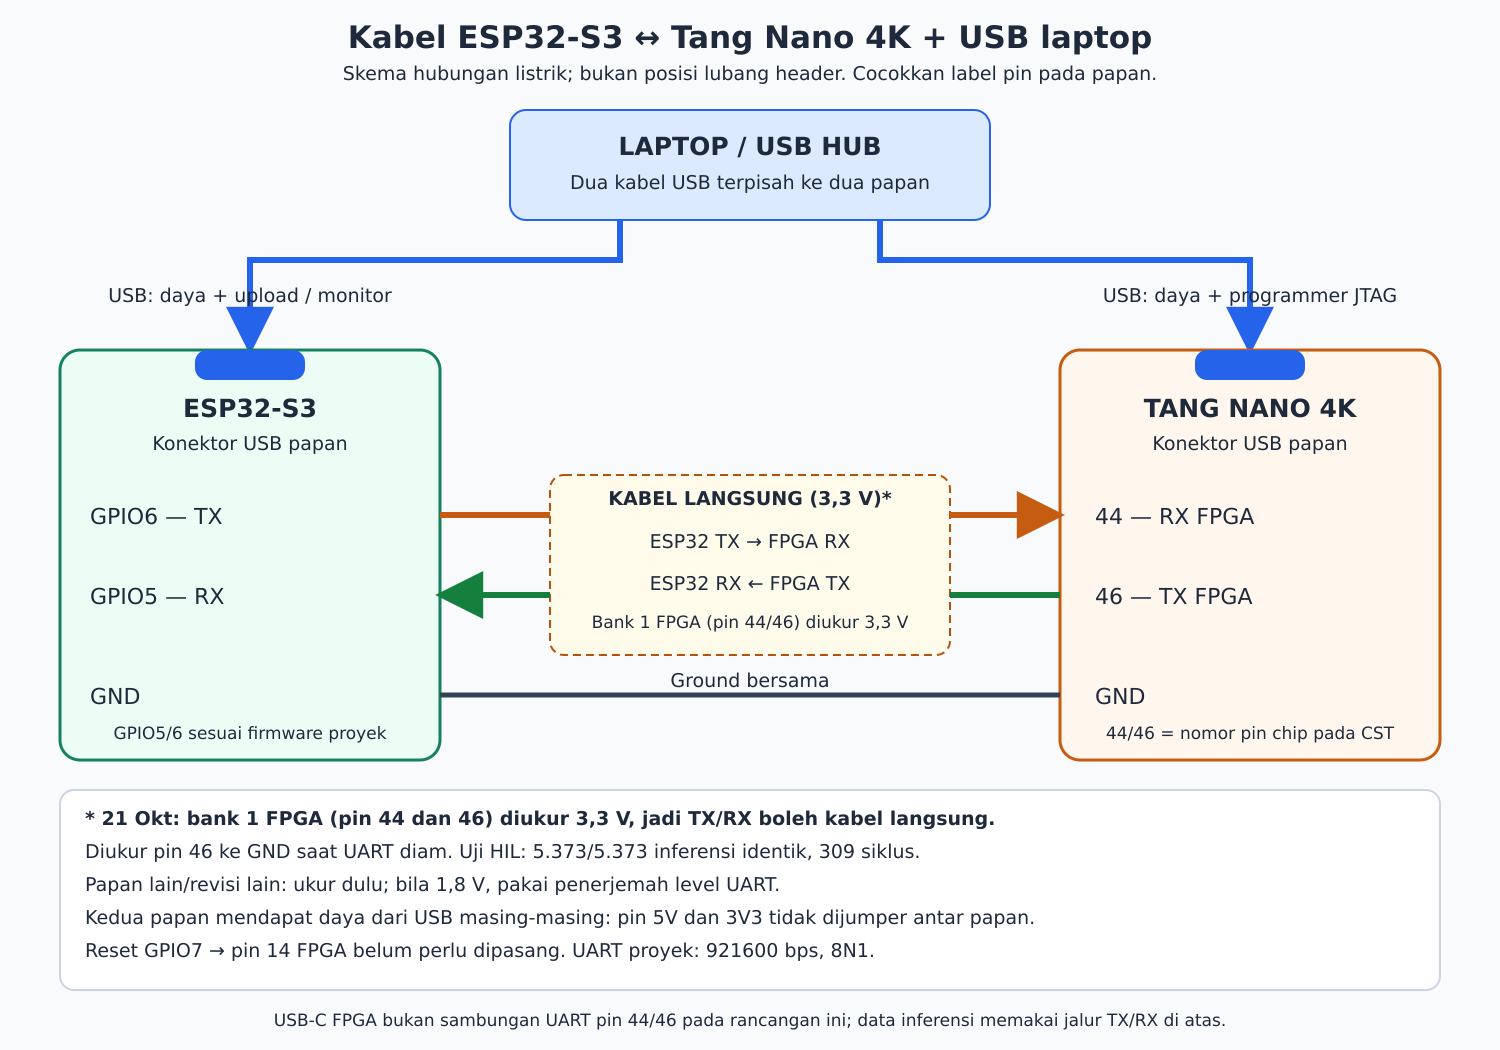
\includegraphics[width=\linewidth]{../../demo/kabel-esp32s3-fpga.png}\\[3pt]
{\tiny\ttfamily TX AA 55 00 00 00 00 00 00 00 04 0B 00 00 00 74 CC 16 26 88\\RX 55 AA 00 00 01 35 9E \normalfont(status OK, prediksi 0, 309 siklus, CRC cocok)}
\end{column}
\end{columns}
\end{frame}

% ======================================================================
\begin{frame}{Edge node di turbin: ESP32-S3 + FPGA\kriteria{fungsional prototipe}}
\begin{columns}[T]
\begin{column}{0.55\linewidth}
\centering
\resizebox{\linewidth}{!}{\begin{tikzpicture}[every node/.style={font=\scriptsize}]
  \node[milik=genis, text width=2.3cm] (sen) at (0,0) {PZEM-017\\stasiun cuaca\\anemometer};
  \node[milik=genis, text width=3.1cm] (esp) at (4,0) {\textbf{ESP32-S3}\\bersihkan data\\rata-rata 1 menit\\16 fitur INT8\\status + baterai};
  \node[milik=alif, text width=2.3cm] (fpga) at (8,0) {\textbf{Tang Nano 4K}\\MLP INT8\\309 siklus};
  \node[abu, text width=2.3cm] (om) at (0,-2.2) {Open-Meteo\\1$\times$ ambil = 3 hari};
  \node[milik=izma, text width=3.1cm] (net) at (4,-2.2) {MQTT \texttt{WEC/esp32/*}\\antrean flash $\pm$2 hari};
  \node[milik=shania, text width=2.3cm] (rel) at (8,-2.2) {relai PLN\\dump load};
  \draw[panah] (sen) -- node[label, above=2pt]{RS-485} (esp);
  \draw[panah] ([yshift=4pt]esp.east) -- node[label, above=1pt]{19 B + CRC} ([yshift=4pt]fpga.west);
  \draw[panah] ([yshift=-4pt]fpga.west) -- node[label, below=1pt]{7 B + CRC} ([yshift=-4pt]esp.east);
  \draw[panah] (esp) -- (net);
  \draw[panah] (esp.south east) -- (rel.north west);
  \draw[putus] (om.north east) -- (esp.south west);
\end{tikzpicture}}\\[6pt]
\scriptsize Kalau FPGA tidak menjawab dalam 20 ms, ESP32 menghitung MLP yang sama (bit-exact) dan mencatat \texttt{n\_beda}.
\end{column}
\begin{column}{0.43\linewidth}
\small\textbf{Diuji di laptop (C++ inti = firmware)}\\[3pt]
\scriptsize
\begin{tabularx}{\linewidth}{@{}X r@{}}
\toprule
MLP (2 model) vs golden & 0 beda (1.197) \\
32 fitur dari riwayat vs Python & 0 beda (400) \\
Baterai vs mesin Node-RED & 0 beda (2.000) \\
Paket UART + CRC-8 vs RTL 21 Okt & 0 beda (600) \\
Build ESP32-S3 N16R8 & RAM 31\%, flash 13\% \\
\bottomrule
\end{tabularx}\\[6pt]
\small\textbf{Di papan (21 Okt):} UART ke FPGA lulus HIL (5.373/5.373). \textbf{Belum:} sensor Modbus dan relai.
\end{column}
\end{columns}
\end{frame}

% ======================================================================
\begin{frame}[label=lebihmaju]{Lebih maju: sampai baterai dan AC\kriteria{inovasi \& kebaruan}}
\begin{columns}[T]
\begin{column}{0.55\linewidth}
\resizebox{\linewidth}{!}{\diagram{baterai}}
\end{column}
\begin{column}{0.43\linewidth}
\footnotesize
\begin{itemize}
  \item \textbf{Edge, tanpa internet}: prediksi dan data tetap ada saat internet mati (Raspi kini reboot tiap internet putus).
  \item \textbf{Tahan sensor mati}: PZEM diam $\to$ daya diganti daya wajar dari angin; MAE \textbf{5,14 W} vs 5,07 W normal (persistence 7,20 W).
  \item \textbf{Tahan data berlubang}: 20\% menit hilang (Raspi reboot) $\to$ prediksi tetap ada \textbf{97,7\%} waktu, MAE 5,07 vs 5,00 W.
  \item \textbf{Interval P10--P90}, bukan satu angka.
  \item \textbf{Rantai ke baterai/AC}: prediksi energi masuk baterai, SoC 1 jam, dan peringatan impor PLN.
  \item Data yang \textbf{harus diukur}: V/I baterai, SoC, suhu, keluaran inverter, dump load. \textbf{Dari publik}: kurva inverter CEC, dataset baterai NASA/CALCE.
\end{itemize}
\IfFileExists{../data/baterai_ringkas.tex}{\scriptsizeSimulasi Okt: galat SoC 1 jam 1,12 poin (MLP INT8) vs 1,82 poin (persistence).}{}
\end{column}
\end{columns}
\end{frame}

% ======================================================================
\begin{frame}[label=bisnis]{Model bisnis dan substitusi impor\kriteria{TKDN \& ekosistem lokal (10\%)}}
\begin{columns}[T]
\begin{column}{0.47\linewidth}
\small
\textbf{Siapa membayar}
\begin{itemize}\scriptsize
  \item Pengelola PLTB/PLTH kecil dan pembangkit tersebar (off-grid, hibrida, kampus, BTS).
  \item Integrator EBT dan BUMN energi (mis.\ Len) $\to$ modul masuk paket proyek.
  \item PLN Puslitbang: pilot riset \emph{prediksi setelah inverter/baterai}.
\end{itemize}
\textbf{Pendapatan} (urutan validasi)
\begin{enumerate}\scriptsize
  \item Pilot + jasa integrasi per lokasi.
  \item Modul per turbin + dukungan tahunan (dashboard, pembaruan model).
  \item Lisensi IP core akselerator ke OEM / mitra semikonduktor.
\end{enumerate}
{\scriptsize Harga belum dikunci sebelum 5--8 wawancara calon pengguna (rencana BMC).}
\end{column}
\begin{column}{0.51\linewidth}
\small\textbf{Komponen inti per turbin} {\scriptsize(harga RAB, Tokopedia, Okt 2026)}\\[2pt]
\scriptsize
\begin{tabularx}{\linewidth}{@{}X r@{}}
\toprule
ESP32-S3-DevKitC-1 N16R8 & Rp144.900 \\
Modul RS-485 terisolasi & Rp139.125 \\
Tang Nano 4K (FPGA) & $\pm$Rp300.000$^{*}$ \\
PCB carrier 2 lapis (cetak lokal) & Rp39.900 \\
\midrule
\textbf{Edge node} & \textbf{$\approx$Rp624.000} \\
Pembanding: Orange Pi 3B + microSD + casing + adaptor & Rp3.294.795 \\
\bottomrule
\end{tabularx}
{\tiny $^{*}$ perkiraan dari harga ritel luar negeri (US\$18--21); belum ada di RAB.}\\[4pt]
\textbf{Substitusi impor bertahap}
\begin{tabularx}{\linewidth}{@{}l X@{}}
Sekarang & IP core RTL, firmware, model, dashboard \textbf{milik sendiri}; papan masih impor \\
Produk & PCB rancangan sendiri, dirakit EMS lokal; server sendiri (bukan SaaS asing) \\
Lanjut & IP core yang sama ke ASIC (MPW) $\to$ ganti NPU/SBC impor \\
\end{tabularx}
\end{column}
\end{columns}
\end{frame}

% ======================================================================
\begin{frame}[label=hilirisasi]{Hilirisasi dan dampak\kriteria{dampak 15\% \textbullet{} hilirisasi 10\%}}
\begin{columns}[T]
\begin{column}{0.5\linewidth}
\textbf{Peta jalan}
\begin{center}
\begin{tikzpicture}[x=1.05cm, every node/.style={font=\scriptsize}]
  \draw[line width=1pt, izma, -{Stealth}] (0,0) -- (6.2,0);
  \foreach \x/\t/\b in {0/Okt 2026/{\textbf{sekarang: TKT 5}\\live di lapangan\\+ chip di papan}, 2/Des 2026/{target TKT 6\\edge node di turbin\\+ baterai, 1 bulan}, 4/2027/{target TKT 7\\pilot mitra\\2--3 lokasi}, 6/2028/{target TKT 8\\produk + uji\\kualifikasi, ASIC}}
    {\fill[izma] (\x,0) circle (2.5pt); \node[above=3pt, font=\scriptsize\bfseries] at (\x,0) {\t}; \node[below=3pt, align=center] at (\x,0) {\b};}
\end{tikzpicture}
\end{center}
\small
\begin{itemize}
  \item Sasaran: pengelola pembangkit terbarukan tersebar; RUPTL 2025--2034 menargetkan +7,2 GW angin.
  \item Calon mitra: \textbf{PLN Puslitbang} (pilot prediksi setelah inverter/baterai), \textbf{PT Len} (integrasi EBT), lab CITA ITB (lokasi uji).
  \item Modul per turbin $\approx$Rp624 rb (ESP32-S3 + FPGA kecil).
\end{itemize}
\end{column}
\begin{column}{0.48\linewidth}
\textbf{TKDN dan kekayaan intelektual}
\small
\begin{itemize}
  \item RTL akselerator, golden model, dan pipeline data \textbf{milik sendiri} (open toolchain Yosys/nextpnr).
  \item FPGA bisa diprogram ulang untuk fitur baru (mis.\ sensor getaran) tanpa ganti chip.
  \item Rancangan yang sama dilanjutkan ke ASIC (OpenLane + SKY130).
\end{itemize}
\end{column}
\end{columns}
\end{frame}

% ======================================================================
\begin{frame}[label=status]{Status purwarupa: apa yang sudah jalan\kriteria{fungsional prototipe}}
\footnotesize
\begin{tabularx}{\linewidth}{@{}l l X@{}}
\toprule
Bagian & Status & Bukti \\
\midrule
Sensor atap $\to$ Raspi $\to$ MQTT $\to$ Node-RED & \textcolor{genis}{\textbf{live}} & dashboard \texttt{/hackathon}; data 181 rb menit + InfluxDB \\
Mesin ML 3 fitur (MLP INT8 = FPGA) & \textcolor{genis}{\textbf{live}} & tiap menit; tahan PZEM diam (MAE 5,14 W) dan data berlubang (cakupan 97,7\%) \\
Akselerator MAC4 di Tang Nano 4K & \textcolor{genis}{\textbf{jalan di papan}} & HIL ESP32-S3 $\leftrightarrow$ FPGA: 5.373/5.373 identik, 309 siklus \\
Data live $\to$ chip $\to$ dashboard & \textcolor{genis}{\textbf{live}} & ESP32-S3 $\to$ Tang Nano 4K tiap menit; hasil chip tampil di dashboard \\
Firmware ESP32-S3 & \textcolor{alif}{\textbf{siap}} & build lulus; inti C++ 0 beda vs Python/JS; belum dirakit \\
Baterai, inverter, relai & \textcolor{lama}{\textbf{simulasi}} & model aki 12 V 50 Ah + kurva inverter CEC; perlu sensor V/I baterai \\
\bottomrule
\end{tabularx}\\[8pt]
\begin{tikzpicture}
  \node[draw=shania, fill=shania!8, rounded corners=4pt, text width=13cm, align=center, font=\small, inner sep=5pt]
  {Satu sumber bobot (\texttt{ml/.../export}) dipakai FPGA, ESP32, Node-RED, dan browser $\to$ hasil identik bit demi bit di semua lapis.};
\end{tikzpicture}
\end{frame}

% ======================================================================
\begin{frame}{Rencana tiga hari hackathon}
\centering
\begin{tikzpicture}[x=3.6cm, y=0.62cm, every node/.style={font=\small}]
  \foreach \i/\d/\s in {0/Hari 1 (21 Okt)/Explore \& Define, 1/Hari 2 (22 Okt)/Build \& Improve, 2/Hari 3 (23 Okt)/{Pitch \textbullet{} Blok A 09.20}}
    {\node[font=\small\bfseries] at (\i+0.5,6.4) {\d}; \node[font=\scriptsize] at (\i+0.5,5.85) {\s}; \draw[black!20] (\i,0) -- (\i,5.5);}
  \draw[black!20] (3,0) -- (3,5.5);
  \foreach \y/\t/\a/\b/\c in {5/Uji HIL FPGA (USB-TTL)/0/0.8/alif, 4/Rakit ESP32-S3 + RS-485 (firmware siap)/0/1.4/genis, 3/ESP32 $\leftrightarrow$ FPGA lewat UART/0.8/1.9/alif,
                               2/Dashboard live + data PZEM pulih/0/1.6/genis, 1/Wawancara + energi per prediksi/0.4/1.9/shania, 0/Deck final (kumpul 22 Okt 23.50) + pitching/1.3/2.6/izma}
    {\fill[\c!55] (\a,\y-0.33) rectangle (\b,\y+0.33); \node[anchor=east, font=\scriptsize] at (0,\y) {\t};}
\end{tikzpicture}\\[4pt]
{\scriptsize Mentoring: H1 14.00 STEI (diagram blok \& rencana chip), 14.40 Len (masalah \& 3 pertanyaan) \textbullet{} H2 11.24 bisnis, 11.36 \& 14.00 PLN, 11.48 Indismart, 13.48 STEI, 14.48 Len}
\end{frame}

% ======================================================================
\begin{frame}[plain,t,label=penutup]
\begin{tikzpicture}[remember picture, overlay]
  \fill[espresso] (current page.north west) rectangle ([yshift=-3.4cm]current page.north east);
  \fill[alif] ([yshift=-3.4cm]current page.north west) rectangle ([yshift=-3.52cm]current page.north east);
  \node[text=krem, font=\fontsize{30}{34}\selectfont\bfseries] at ([yshift=-1.35cm]current page.north) {Terima kasih};
  \node[text=krem!85, font=\large] at ([yshift=-2.4cm]current page.north) {Wind Edge Chip --- prediksi di turbin, hemat daya, milik sendiri};
  \node[milik=alif, text width=3.6cm, text=teks] (b) at ([yshift=-5.0cm]current page.north) {\textbf{309 siklus}\\$\approx$11,4\,$\mu$s / prediksi};
  \node[milik=izma, text width=3.6cm, text=teks, left=0.5cm of b] {\textbf{RMSE 10,25 W}\\skill +0,40};
  \node[milik=genis, text width=3.6cm, text=teks, right=0.5cm of b] {\textbf{181 rb menit}\\data lapangan nyata};
  \node[font=\small, text=teks] at ([yshift=-6.4cm]current page.north) {Dashboard live: \href{http://citaitb.com:1880/dashboard/hackathon}{\color{izma}\texttt{citaitb.com:1880/dashboard/hackathon}}};
\end{tikzpicture}
\end{frame}

% ======================================================================
\appendix
\begin{frame}{Lampiran A --- Aturan preprocessing}
\small
\begin{tabularx}{\linewidth}{@{}X X@{}}
\toprule
Temuan & Tindakan \\
\midrule
Sel $>$45.000 (nomor seri tanggal Excel) & NaN; Daya = V$\times$I bila V, I utuh \\
\texttt{OFF} 61\% baris & 0 W + fitur \texttt{turbin\_on} \\
Angin Arduino macet 1,25 m/s & dibuang; pakai angin stasiun \\
Angin stasiun $>$ 8 m/s (daya median 0 W) & NaN \\
Arah $-115$ saat angin tenang & NaN (arah lain $-114\ldots244$ sah, sensor ber-offset) \\
Spike daya $>$ V$^2$/35\,$\Omega$ & NaN \\
Duplikat/timestamp mundur & urutkan, buang \\
Celah $>$ 10 menit & tidak diinterpolasi; sampel lintas celah dibuang \\
Waktu WIB & disimpan UTC \\
\bottomrule
\end{tabularx}
\end{frame}

\begin{frame}{Lampiran B --- Fitur, target, dan split}
\centering\resizebox{0.85\linewidth}{!}{\diagram{jendela}}\\[6pt]
\small
\begin{tabularx}{\linewidth}{@{}l X@{}}
\toprule
16 fitur & \texttt{p\_now, p\_lag5, p\_lag15, p\_lag30, p\_lag60, p\_mean60, w\_now, w\_mean10, w\_mean60, w3\_mean10, dir\_sin, dir\_cos, hour\_sin, hour\_cos, rho, om\_wind\_next} \\
Target & rata-rata daya $t{+}1\ldots t{+}60$ \\
Split kronologis & latih 30 Mar--31 Jul (99.260) \textbullet{} validasi Agu--Sep (31.700) \textbullet{} uji 1--20 Okt (16.255) \\
Kuantisasi & $x_q = \mathrm{clamp}(\mathrm{round}((x-c)/s), -128, 127)$; keluaran $\times$ 0,972 W \\
\bottomrule
\end{tabularx}
\end{frame}

\begin{frame}{Lampiran C --- Tabel lengkap perbandingan metode}
\IfFileExists{../data/tabel_benchmark_deck.tex}{{\scriptsize\begin{minipage}[t]{0.49\linewidth}\setlength{\tabcolsep}{3pt}\begin{tabular}{@{}r p{4.1cm} r r@{}}
\toprule
\# & Metode & RMSE & Skill \\ \midrule
1 & Transformer (riwayat 60 menit) & 10,07 & +0,411 \\
2 & Regresi linear & 10,23 & +0,402 \\
3 & Ridge & 10,23 & +0,402 \\
4 & TCN (riwayat 60 menit) & 10,25 & +0,401 \\
5 & MLP float 16-8-1 & 10,25 & +0,401 \\
6 & \textbf{MLP INT8 (QAT, identik RTL)} & 10,25 & +0,401 \\
7 & Lasso & 10,25 & +0,401 \\
8 & ElasticNet & 10,25 & +0,401 \\
9 & LSTM (riwayat 60 menit) & 10,35 & +0,395 \\
10 & GRU (riwayat 60 menit) & 10,41 & +0,392 \\
11 & MLP float 16-16-1 & 10,41 & +0,392 \\
12 & MLP float 16-32-16-1 (acuan QAT, train\_mlp.py) & 10,44 & +0,390 \\
13 & CNN 1D (riwayat 60 menit) & 10,46 & +0,389 \\
14 & MLP float 16-32-16-1 & 10,47 & +0,388 \\
15 & MLP float 16-64-32-1 & 10,49 & +0,387 \\
16 & ExtraTrees & 10,59 & +0,382 \\
17 & KNN (k=25) & 10,62 & +0,380 \\
18 & MLP INT8 (PTQ: dibulatkan tanpa QAT) & 10,65 & +0,378 \\
\bottomrule
\end{tabular}\end{minipage}\hfill\begin{minipage}[t]{0.49\linewidth}\setlength{\tabcolsep}{3pt}\begin{tabular}{@{}r p{4.1cm} r r@{}}
\toprule
\# & Metode & RMSE & Skill \\ \midrule
19 & ARIMA(2,0,1) deret 10 menit* & 10,77 & +0,391 \\
20 & Polinomial derajat 2 + Ridge & 10,87 & +0,365 \\
21 & Random Forest & 10,91 & +0,363 \\
22 & campuran mean60 + klimatologi (a=0.35) & 11,00 & +0,357 \\
23 & LightGBM tanpa Open-Meteo (offline) & 11,03 & +0,355 \\
24 & LightGBM kuantil P50 (+ interval P10–P90) & 11,12 & +0,350 \\
25 & LightGBM & 11,16 & +0,348 \\
26 & SVR RBF (15 rb sampel) & 11,23 & +0,344 \\
27 & HistGradientBoosting & 11,27 & +0,341 \\
28 & XGBoost & 11,40 & +0,334 \\
29 & CatBoost & 11,47 & +0,330 \\
30 & Decision Tree & 11,58 & +0,323 \\
31 & Kurva daya $\times$ angin 60 menit terakhir & 12,38 & +0,277 \\
32 & smart persistence (rata-rata 60 menit terakhir) & 12,62 & +0,262 \\
33 & klimatologi per jam & 12,89 & +0,247 \\
34 & moving average 10 menit & 14,39 & +0,159 \\
35 & persistence (P sekarang) & 17,11 & +0,000 \\
36 & Kurva daya $\times$ prakiraan Open-Meteo & 17,19 & -0,005 \\
\bottomrule
\end{tabular}\end{minipage}}}{}
\end{frame}

\begin{frame}{Lampiran D --- Batasan RTL dan catatan integrasi}
\small
\begin{itemize}
  \item Requantize sama untuk semua lapisan: $y = \mathrm{clamp}((\mathrm{acc}\cdot 32) \gg 8, 0, 127)$, ReLU juga di keluaran (daya $\ge$ 0).
  \item Akibatnya bobot hasil latih hanya $\pm5$ dari $\pm127$. Diuji 21 Okt: M per lapisan memakai rentang bobot sampai $\pm45$, tetapi MAE uji tetap 5,45--5,65 W (sebesar selisih antar-pelatihan) $\to$ bukan prioritas RTL.
  \item UART RTL (Alif, 21 Okt): paket 19 B \texttt{[AA 55, 16 fitur, CRC-8]} $\to$ 7 B \texttt{[55 AA, status, prediksi, siklus, CRC-8]}, 921600 bps, watchdog. Firmware ESP32 dan jembatan laptop sudah memakai format ini (uji 600 paket, termasuk CRC rusak: 0 beda).
  \item Verifikasi: PyTorch-QAT = integer numpy = golden model = cermin RTL = RTL Verilog (iverilog: 2.000 acak + 597 nyata + SoC UART), 0 beda. Uji HIL di papan 21 Okt (ESP32-S3 $\leftrightarrow$ Tang Nano 4K): 5.373/5.373 inferensi identik.
  \item Cadangan bila FPGA gagal: \texttt{mlp\_int8.h} di ESP32 (bit-exact, hasil sama dengan FPGA).
\end{itemize}
\end{frame}

\begin{frame}{Lampiran E --- Fitur 1: status turbin}
\small
\begin{tabularx}{\linewidth}{@{}X r@{}}
\toprule
Percobaan & Hasil \\
\midrule
Reproduksi SVM TA (Cp, D=3 m, angin Arduino, split acak) & 97,6\% (klaim TA 98,22\%) \\
Model asli Raspi, data 16 Jun--20 Okt & 98,2\% \\
Versi perbaikan (angin stasiun, D=2,5 m, kronologis): SVM RBF / RF / LightGBM & 99,1 / 98,8 / 98,7\% \\
Deteksi kurva daya: daya tersisa 20\% (jendela 30 menit) & 68\% terdeteksi, alarm palsu 3,8\% \\
\bottomrule
\end{tabularx}
\vspace{4pt}

Label Cp adalah rumus dari input, sehingga akurasi tinggi berarti model meniru rumus. Pendekatan kurva daya menilai kinerja terhadap daya \emph{wajar} untuk kondisi angin.
\end{frame}

\begin{frame}{Lampiran F --- Bahan mentoring Hari 1}
\begin{columns}[T]
\begin{column}{0.48\linewidth}
\small\textbf{Ringkasan (Len, 14.40)}
\begin{itemize}\scriptsize
  \item \textbf{Masalah:} daya turbin kecil 0 sampai $>$100 W dalam hitungan jam; pengelola tak punya dasar memutuskan isi baterai, beban, atau PLN; data hilang tiap internet mati.
  \item \textbf{Solusi:} prediksi rata-rata daya 1 jam di turbin (MLP INT8 di akselerator FPGA sendiri), status kurva daya, dan prakiraan SoC baterai $\to$ keputusan relai.
  \item \textbf{Bukti:} 181 rb menit data nyata; MAE 5,48 W (persistence 8,67 W); RTL Verilog 0 beda; tetap jalan saat PZEM diam.
\end{itemize}
\end{column}
\begin{column}{0.5\linewidth}
\small\textbf{Tiga pertanyaan untuk mentor}
\begin{enumerate}\scriptsize
  \item Pada sistem PLTB/hibrida yang ditangani Len, keputusan mana yang paling butuh prediksi 1 jam: penjadwalan baterai, pelepasan beban, atau genset/PLN? Berapa galat yang masih bisa diterima?
  \item Syarat apa yang wajib dipenuhi modul edge agar layak pilot (suhu, IP, protokol Modbus/IEC, sertifikasi)?
  \item Untuk TKDN: apakah IP core + PCB rakitan lokal (FPGA masih impor) sudah dihitung, dan Len lebih tertarik membeli modul atau melisensikan IP core?
\end{enumerate}
\small\textbf{Diagram blok (STEI, 14.00):} slide Arsitektur, Chip L3, Model dilatih dengan aritmetika chip, Edge node.
\end{column}
\end{columns}
\end{frame}

\end{document}
